\chapter{INTRODUCTION} \label{ch:introduction}% Must have a blank line after every section label

Who is Jack Handey and how did he become so wise?  Jack's story begins long ago, when he was just a boy in search of answers.  

\section{Jack Handey's Early Years} \label{sec:Jack Early Years} % Must have a blank line after every section label

Young Jack did not appear to be anything special to friends and family.  Of course they loved him because he was family, but few would say they saw early signs of wisdom in the child.  

\begin{figure}[tbph]
\centering
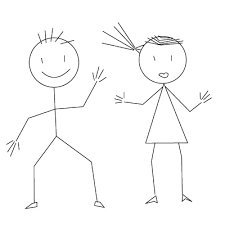
\includegraphics[width=.5\linewidth]{./fig/Dissertation_Image.png} %Include graphic at 1=100 \% linewidth vs textwidth as it will size if put in columns. Textwidth wont resize in columns
\caption{An early piece of artwork by Jack Handey, age 17}
\label{fig:JackArt}
\end{figure} 

Jack's mother saw a glimmer of something in him, however, and sent him to live with monks on the remote island of Bouvet, approximately 1,000 miles from Antarctica.  On this island covered almost entirely by a glacier, laden with sheer cliffs, Jack imbibed the wisdom of these monks and learned to become a font of wisdom himself.

\section{Beyond Bouvet} \label{sec:Beyond Bouvet} % Must have a blank line after every section label
 
After spending 10 years with the monks on Bouvet, they realized that he had learned all that he could from them.  With tears in his eyes, Jack left them with one final piece of wisdom to ponder: 
\begin{quote}
\emph{As you make your way thought this hectic world of ours, set aside a few minutes each day.  At the end of the year, you'll have a couple of days saved up \cite{Handey1994}.}
\end{quote}
With these words, Jack left the frigid wilds of Bouvet and prepared to rejoin the modern world.  Although he would be a keen observer of the human condition, he would never fully become part of society, but rather remained on the fringes as he shared his insights.
